
\documentclass[a4paper,twocolumn]{article}
\usepackage{graphicx}
\usepackage{amsmath}

\title{On-orbit rate normalization}
\author{Luca Baldini (luca.baldini@pi.infn.it)}

\begin{document}

\maketitle

\abstract{This is a short memo on the basic strategy we use to normalize the
on-orbit LAT rates (with several different cuts applied) for the purpose of the
data monitoring and the alarm system. The original implementation of the
necessary code was put in place by David Paneque shortly after the launch.
When we changed the rocking angle from $35^\circ$ to $50^\circ$ I made the
necessary modifications to take into account the rate variations due to the
change of the Earth limb arc length into the instrument field of view
(especially in the selection with the highest photon content, namely the
\emph{source} and \emph{diffuse} classes).

This note describe some of the work involved, along with additional
modifications triggered by an excessive rate of spurious warnings during the
rocking of the instrument that we started getting in the summer of 2010.
The code necessary to produce the configuration files for the normalization
code running in the pipeline is shortly described for future reference.}

\section{Introduction}

As of August 14, 2010, the normalized rates are calculated by the data
monitoring code running in the L1Proc pipeline based on the McIlwainL parameter
and the rocking angle of the instrument. Some more details will be given in the
following section. The purpose of this note is to describe possible
improvements in order to  avoid two specific issues which cause spurious
alarms to trigger with a significant rate.

The first is a recurrent spike in the photon-rich data samples (most notably
the diffuse class) corresponding to the rocking of the instrument
(cfr. figure \ref{DiffuseEvts_old}).
This is due to the fact that, with a rocking profile of $50^\circ$, the LAT
has the Earth limb in the field of view for most of the time---except for the
few minutes per orbit while it's rocking. When that happens, the photon-rich
classes feature a decrease in the corresponding rate which must be properly
taken into account (the contribution of photons from the Earth limb is
negligible in the background-dominated data samples, so this is less of an
issue for the selection with a high background content).
\begin{figure}[htb!]
  \begin{center}
    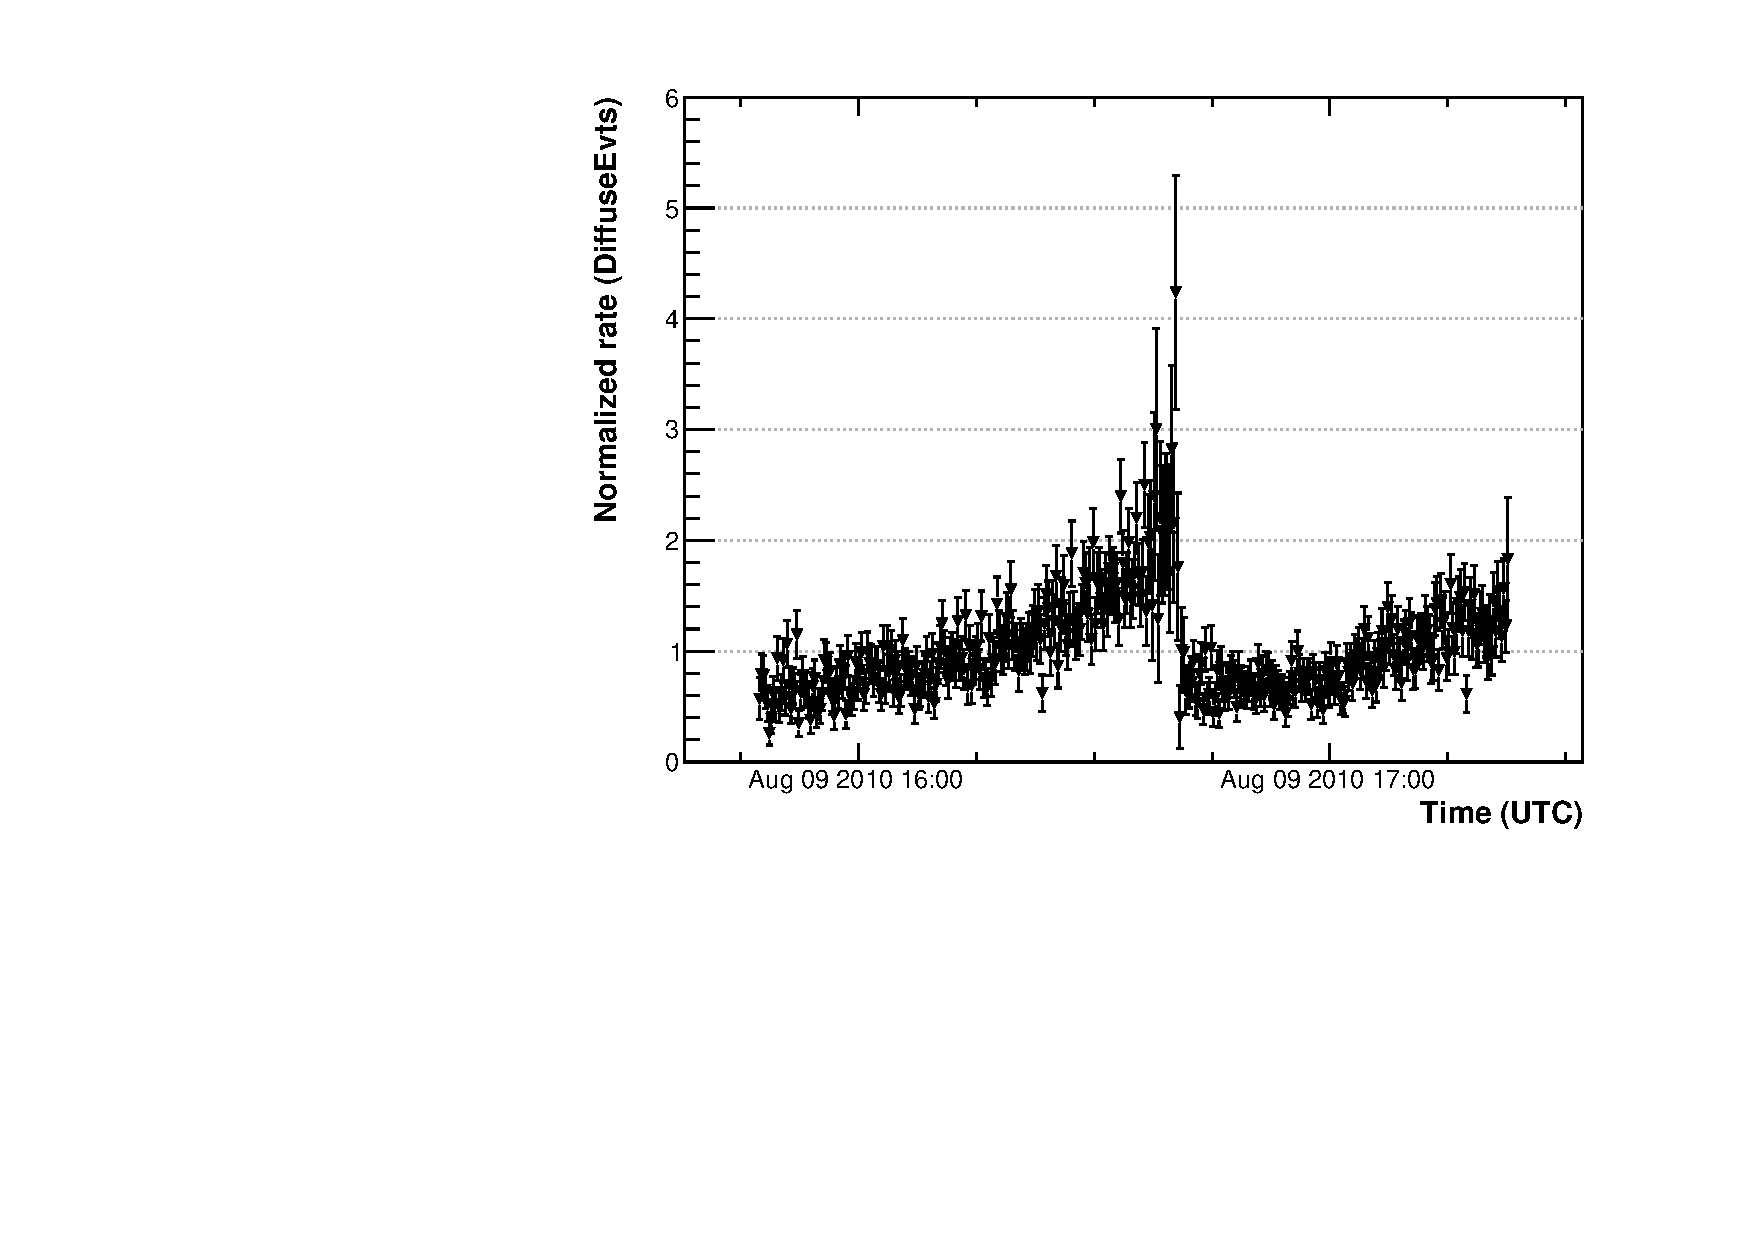
\includegraphics[width=\linewidth]{figures/DiffuseEvts_old}
    \caption{Normalized rate for the diffuse class events for run 0303054436.
      The spike in the middle of the run correspond to the rocking of the
      instrument.}
    \label{DiffuseEvts_old}
  \end{center}
\end{figure}

The second issue is a recurrent dip for the background-dominated data samples
occurring, as we shall see, at a specific longitude in the orbit of the
observatory (cfr. figure \ref{EvtsBeforeCuts_old}) and most likely related
to the South Atlantic Anomaly (in fact the recurrence of the dip is modulated
according to the SAA epoch).
\begin{figure}[htb!]
  \begin{center}
    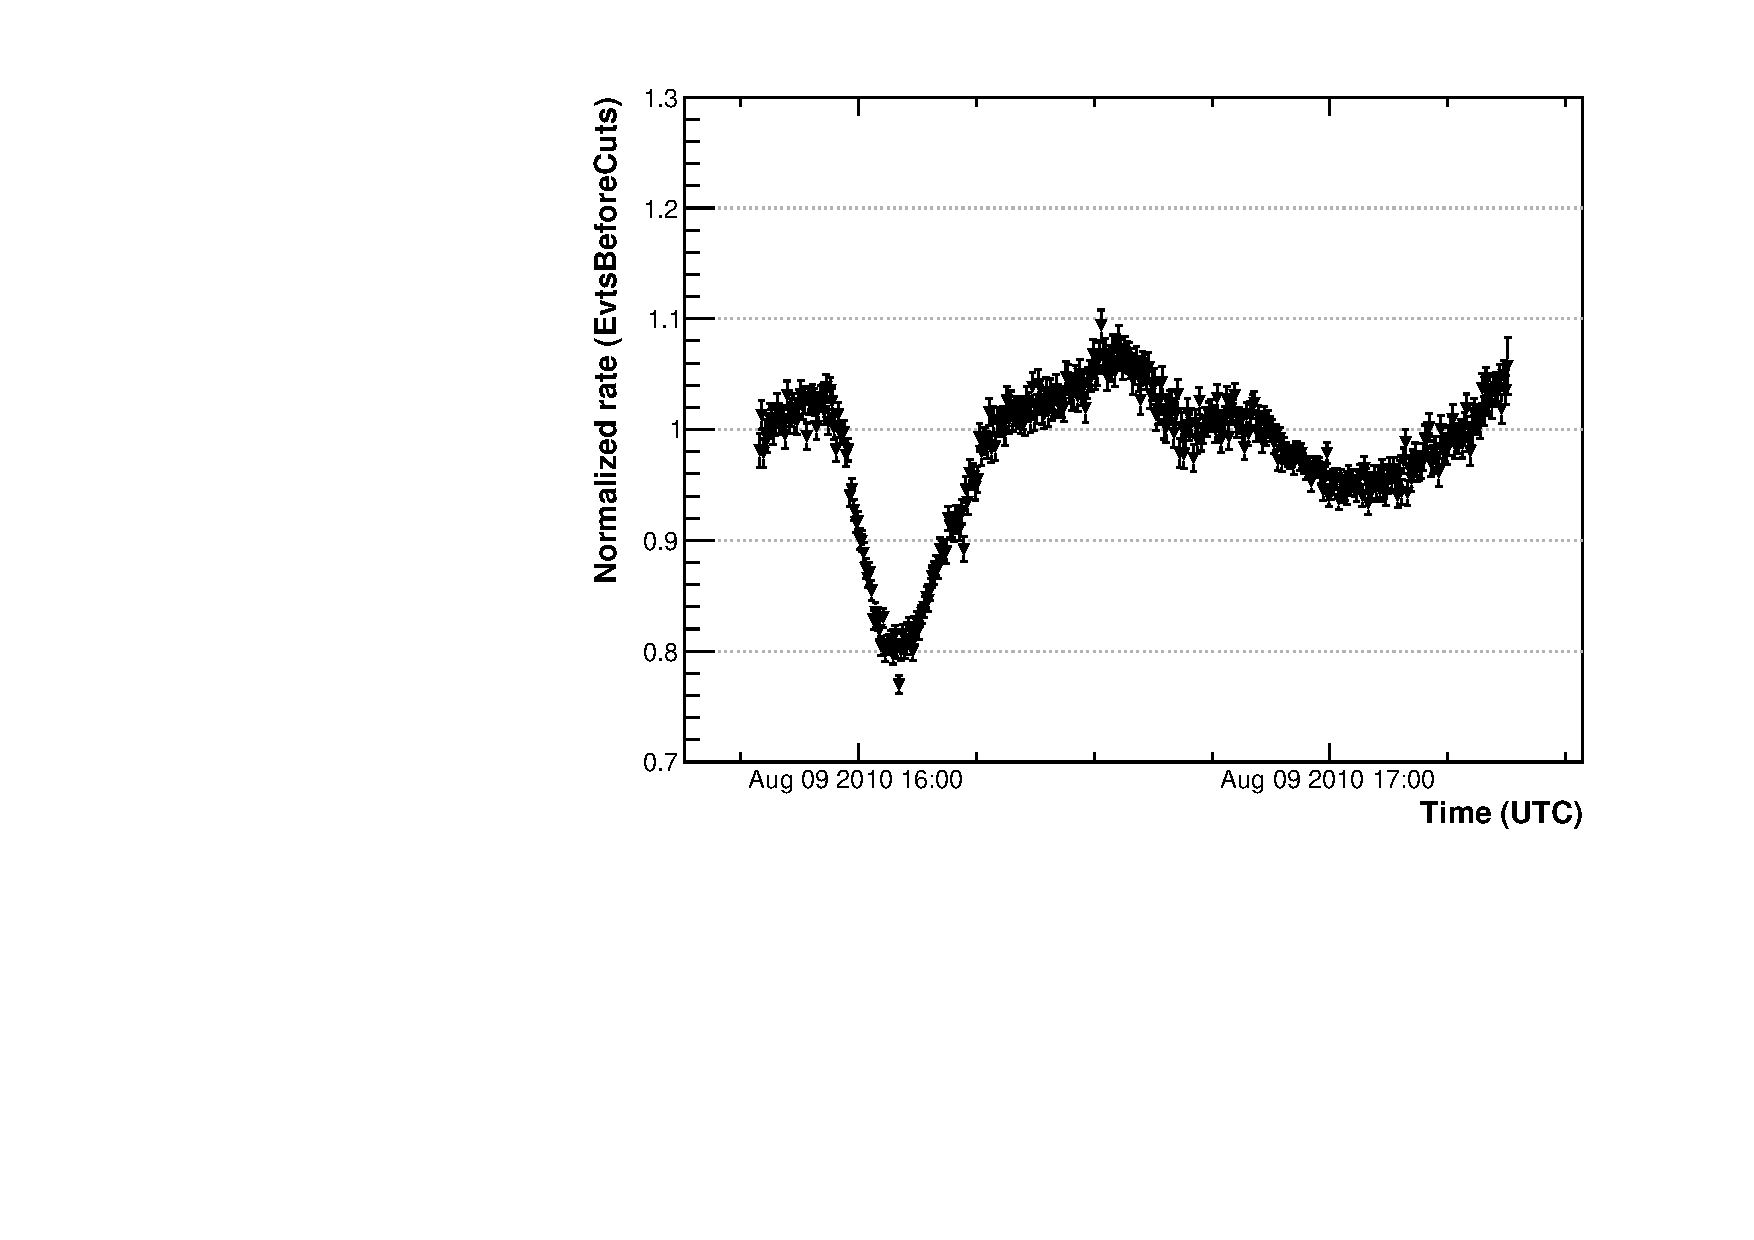
\includegraphics[width=\linewidth]{figures/EvtsBeforeCuts_old}
    \caption{Normalized rate for the events before any cut for run 0303054436.
      As we shall see, the dip close to the beginning of the run is
      characteristic of a particular spot in the orbit and can be (at least
      partially) corrected for.}
    \label{EvtsBeforeCuts_old}
  \end{center}
\end{figure}

Both aspects will be discussed with more details in the following sections.


\section{McIlwain L normalization}

The first (and most prominent) correction is the one taking into account
the McIlwain L geomagnetic parameter.

The starting point is a root tree in which the merit trending product for a
long time span (typically 56 days) are merged together (details on how to
produce such a tree will be given in the next sections).
\begin{figure}[htb!]
  \begin{center}
    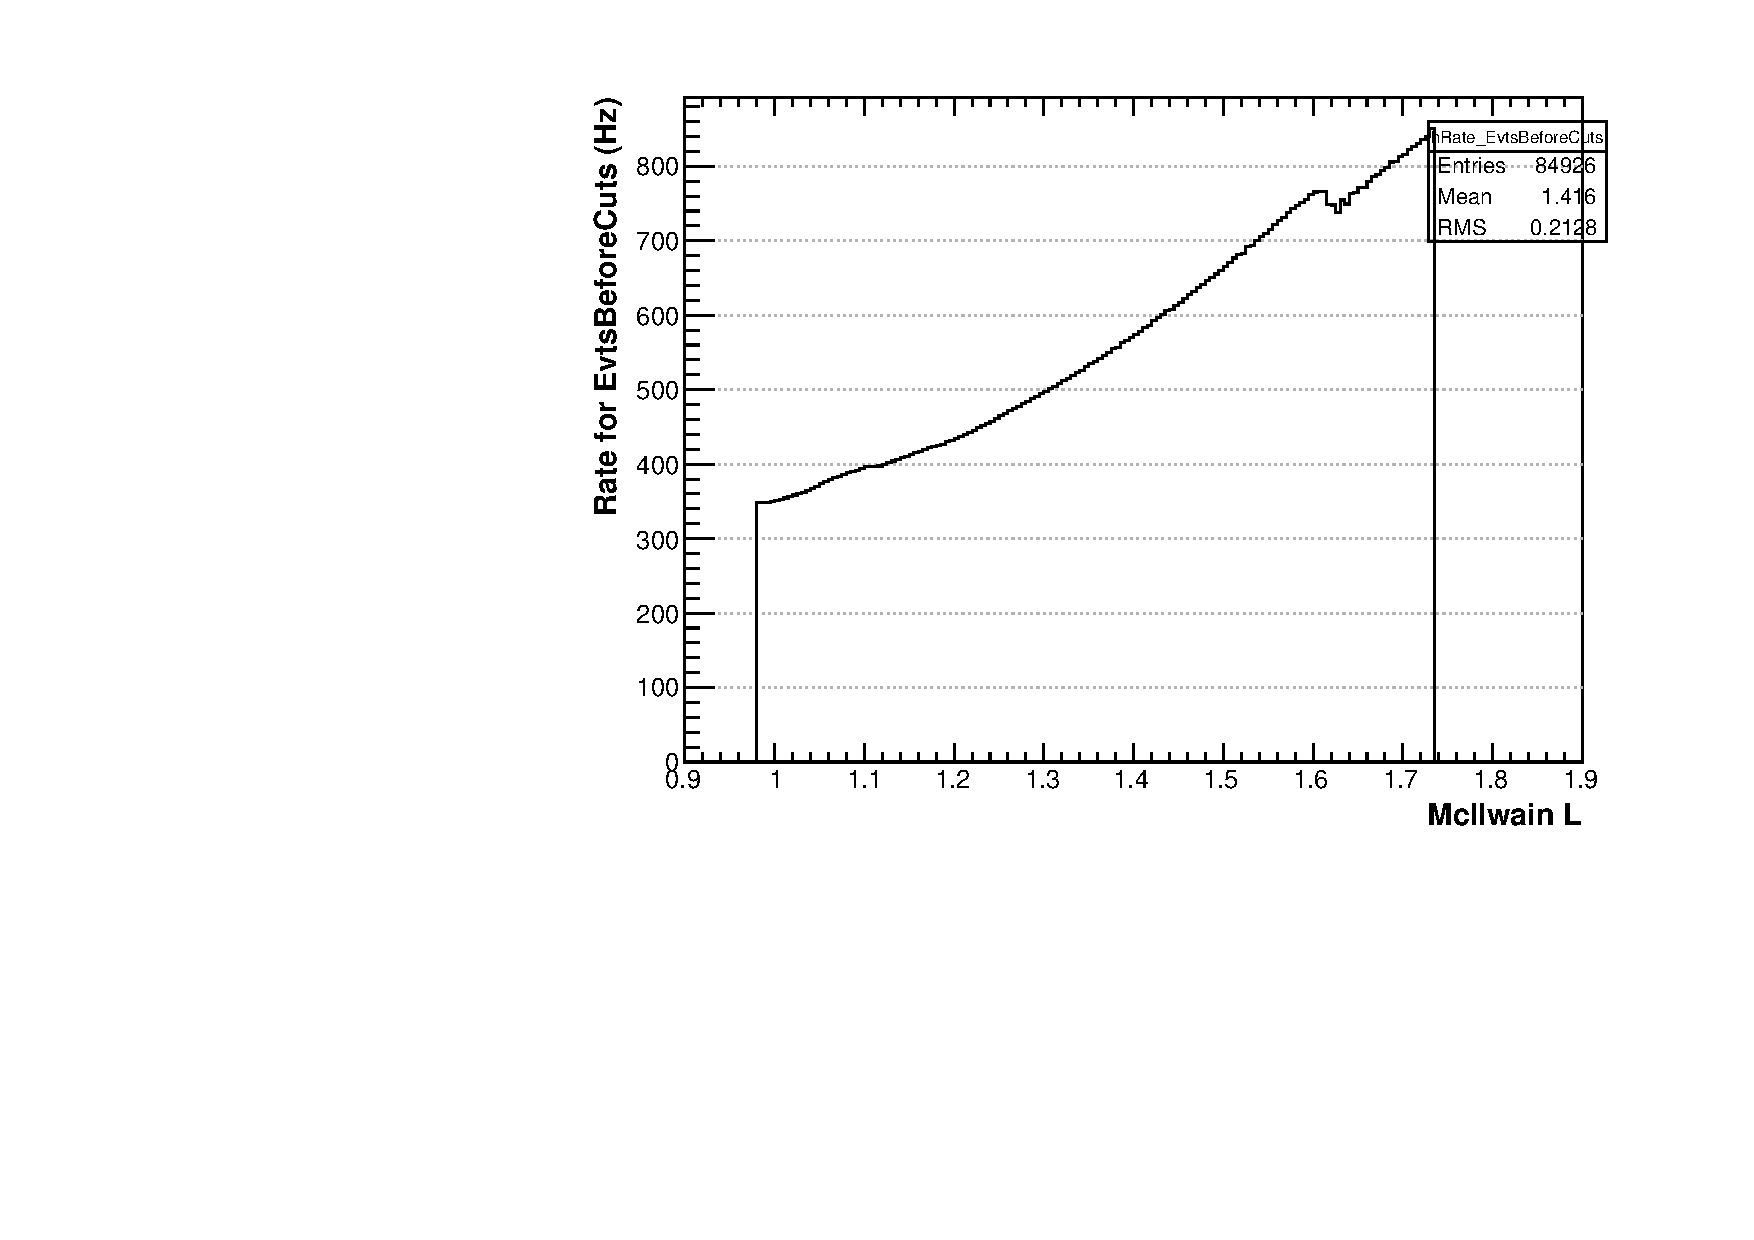
\includegraphics[width=\linewidth]{figures/EvtsBeforeCuts_mcIlwainL}\\
    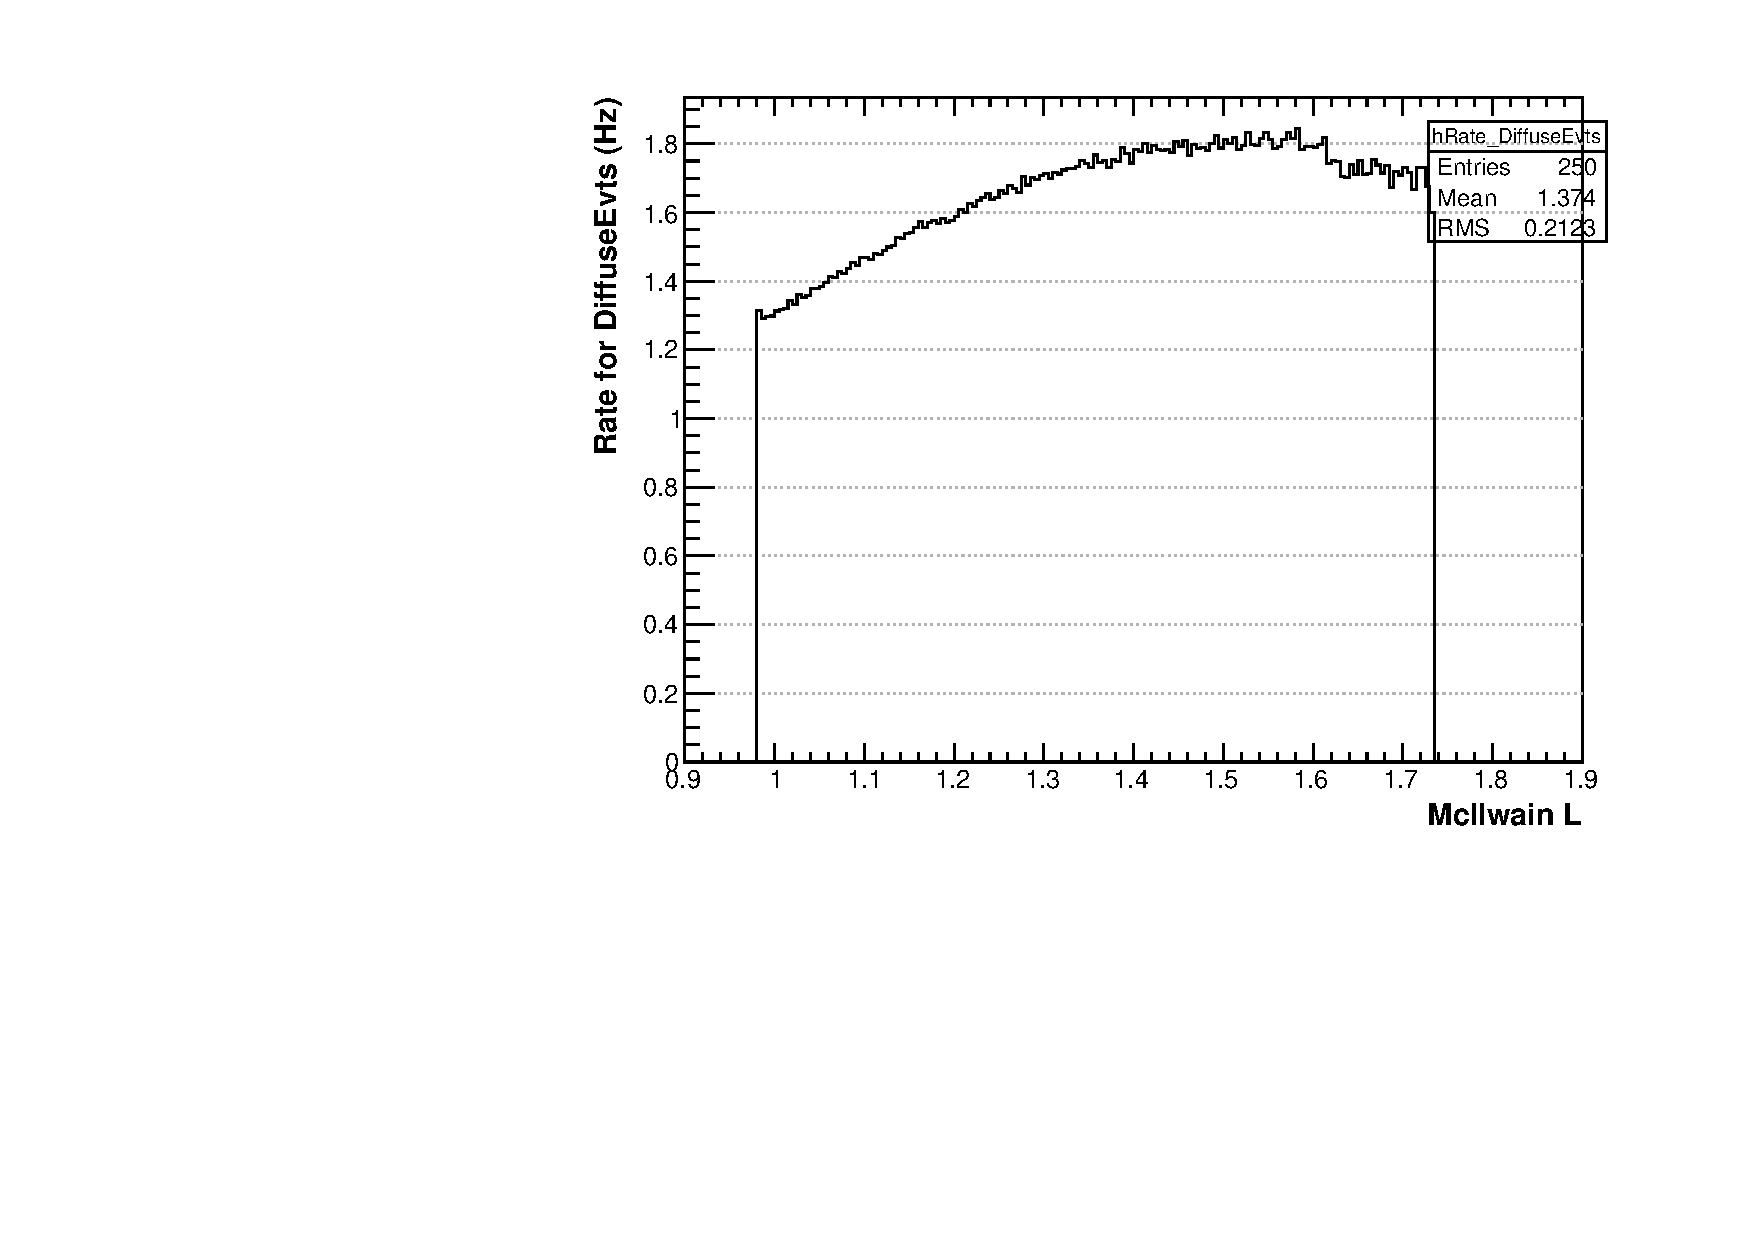
\includegraphics[width=\linewidth]{figures/DiffuseEvts_mcIlwainL}
    \caption{Dependence of the event rate on the McIlwain L parameter for
      two different selections: before any cut (top panel) and after the
      diffuse cuts (bottom panel).}
    \label{mcIlwainL}
  \end{center}
\end{figure}
An histogram of the \texttt{Mean\_PtMcIlwainL} variable
is created requiring that the rocking zenith angle $\theta_r$ is close
(typically within $0.2^\circ$) to $50^\circ$. For each rate variable 
another histogram is made (with the same cut) and the latter is divided by the
first one. The procedure (the result is shown in figure \ref{mcIlwainL} for
two different selections) is equivalent to the calculation of the average rate 
(for each selection) in each McIlwain L bin (with unit weight).

For each bin in such histograms the bin content gives the number the
corresponding rate must be divided by to get the normalized rate (at $50^\circ$
rocking angle) in each McIlwain L bin (for historical reasons the information
in the output text file is stored in the form of a global average value and
the relative bin-to-bin corrections, but this is substantially irrelevant).
The basic idea is that this first step takes care of the geomagnetic
dependence at the typical rocking angle and the additional variations are
taken care of in successive steps.

\section{The Earth limb in the FOV}

Next comes the normalization for the Earth limb in the field of view. In the
original implementation the dependence of the various rates on the rocking
angle (for $\theta_r \neq 50^\circ$) was fitted (with no additional cut) with
a polynomial of third degree.
The choice of the fitting function was, retrospectively, a bad choice, as
in general the best fit featured a concavity in the region
$0^\circ \leq \theta_r \leq 40^\circ$, where the Earth limb is outside the
field of view and therefore the event rates should be approximately constant.
Another issue was due to the fact that for the low-background event classes
(most notably the diffuse class) the absolute average rate is low---typically
of the order of $\approx 0.2$~Hz when the Earth limb is outside the field of
view.
As a consequence the number of counts in a 15~s time bin is also low
($\approx 3$) and the corresponding Poisson fluctuations (especially toward
high values) can be noticeable.

The new implementation constitutes an attempt to overcome this limitation. The
functional form of the new fitting function is:
\begin{equation}
  f(\theta_r) =
  \begin{cases}
    c_0 & \theta_r < 35^\circ\\
    c_0 + c_1 \theta_r + c_2 \theta_r^2 & \theta_r > 35^\circ
  \end{cases}
\end{equation}
i. e. it is a constant when the Earth limb is outside the field of view with the
addition of a second order polynomial to parametrize the effect of the Earth
limb itself. On top of that, a cut of the normalized rate (i. e. rate normalized
for the McIlwain L) is performed before the fit, requiring that the rate itself
is greater than 0.3 (adjustable). This has small or no effect for most of the
event classes and constitutes a rough but effective way to artificially
increase the average for the low-rate classes (i. e. diffuse and source) and
suppress the effect of the Poisson fluctuations toward high values.

An example of such a fit (for the diffuse selection, which at this stage is the
most critical one) is presented in figure \ref{DiffuseEvts_zenith}.
\begin{figure}[htb!]
  \begin{center}
    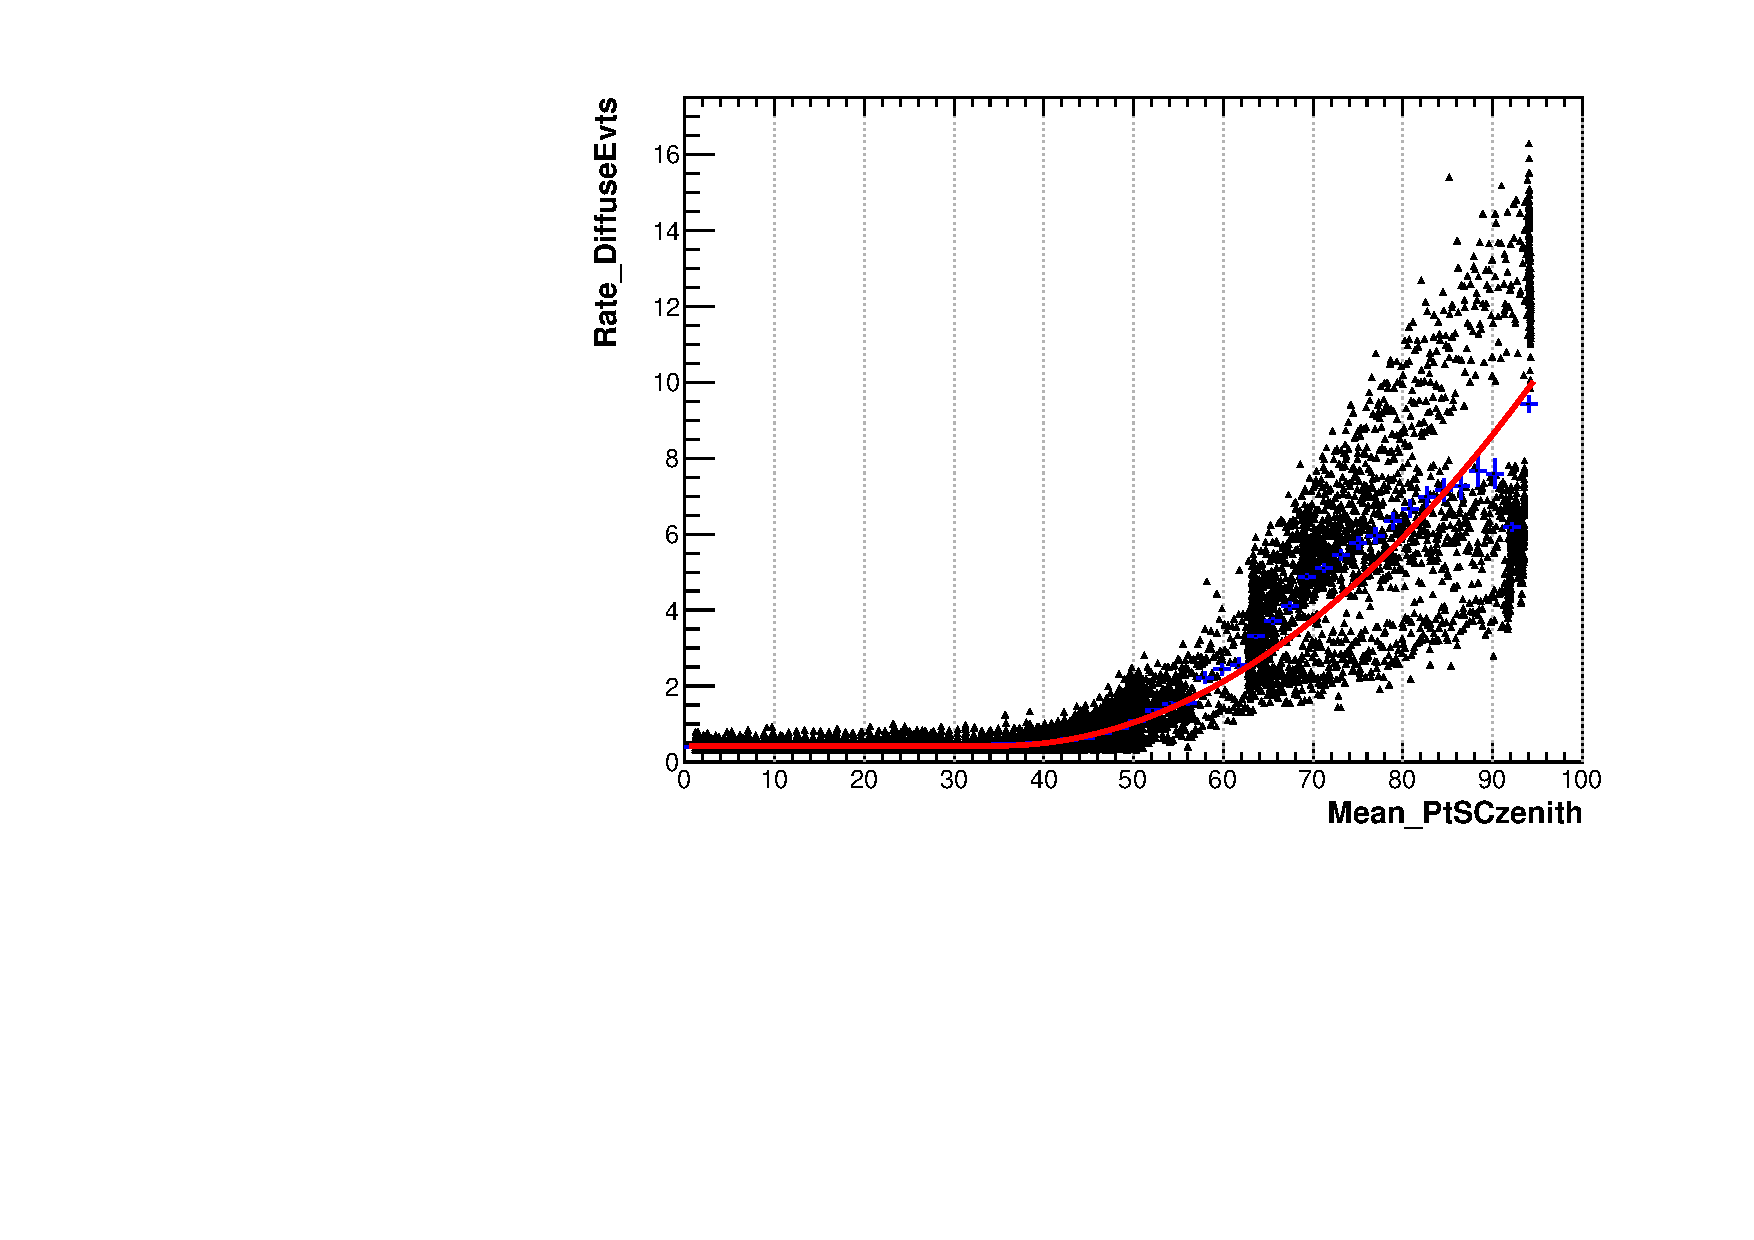
\includegraphics[width=\linewidth]{figures/DiffuseEvts_zenith}
    \caption{Fit of the rocking angle dependence of the diffuse class
      rate (after the normalization for the McIlwain L dependence).
      Each point is a time bin (for a total of 56 days) and the time bins
      with a normalized rate lower than 0.3 have been removed prior to the
      fit. The blue histogram is a profile of the underlying two dimensional
      histogram and the red line is a fit to such a profile.
      Note that the fit value is very close to 1 for $\theta_r = 50^\circ$.}
    \label{DiffuseEvts_zenith}
  \end{center}
\end{figure}

The effect of the new implementation on an actual run is shown in figure
\ref{DiffuseEvts_new}, which can be compared directly with figure
\ref{DiffuseEvts_old}. The improvement is evident, with the highest data point
going down from $\approx 4.5$ to $\approx 2.5$. 
\begin{figure}[htb!]
  \begin{center}
    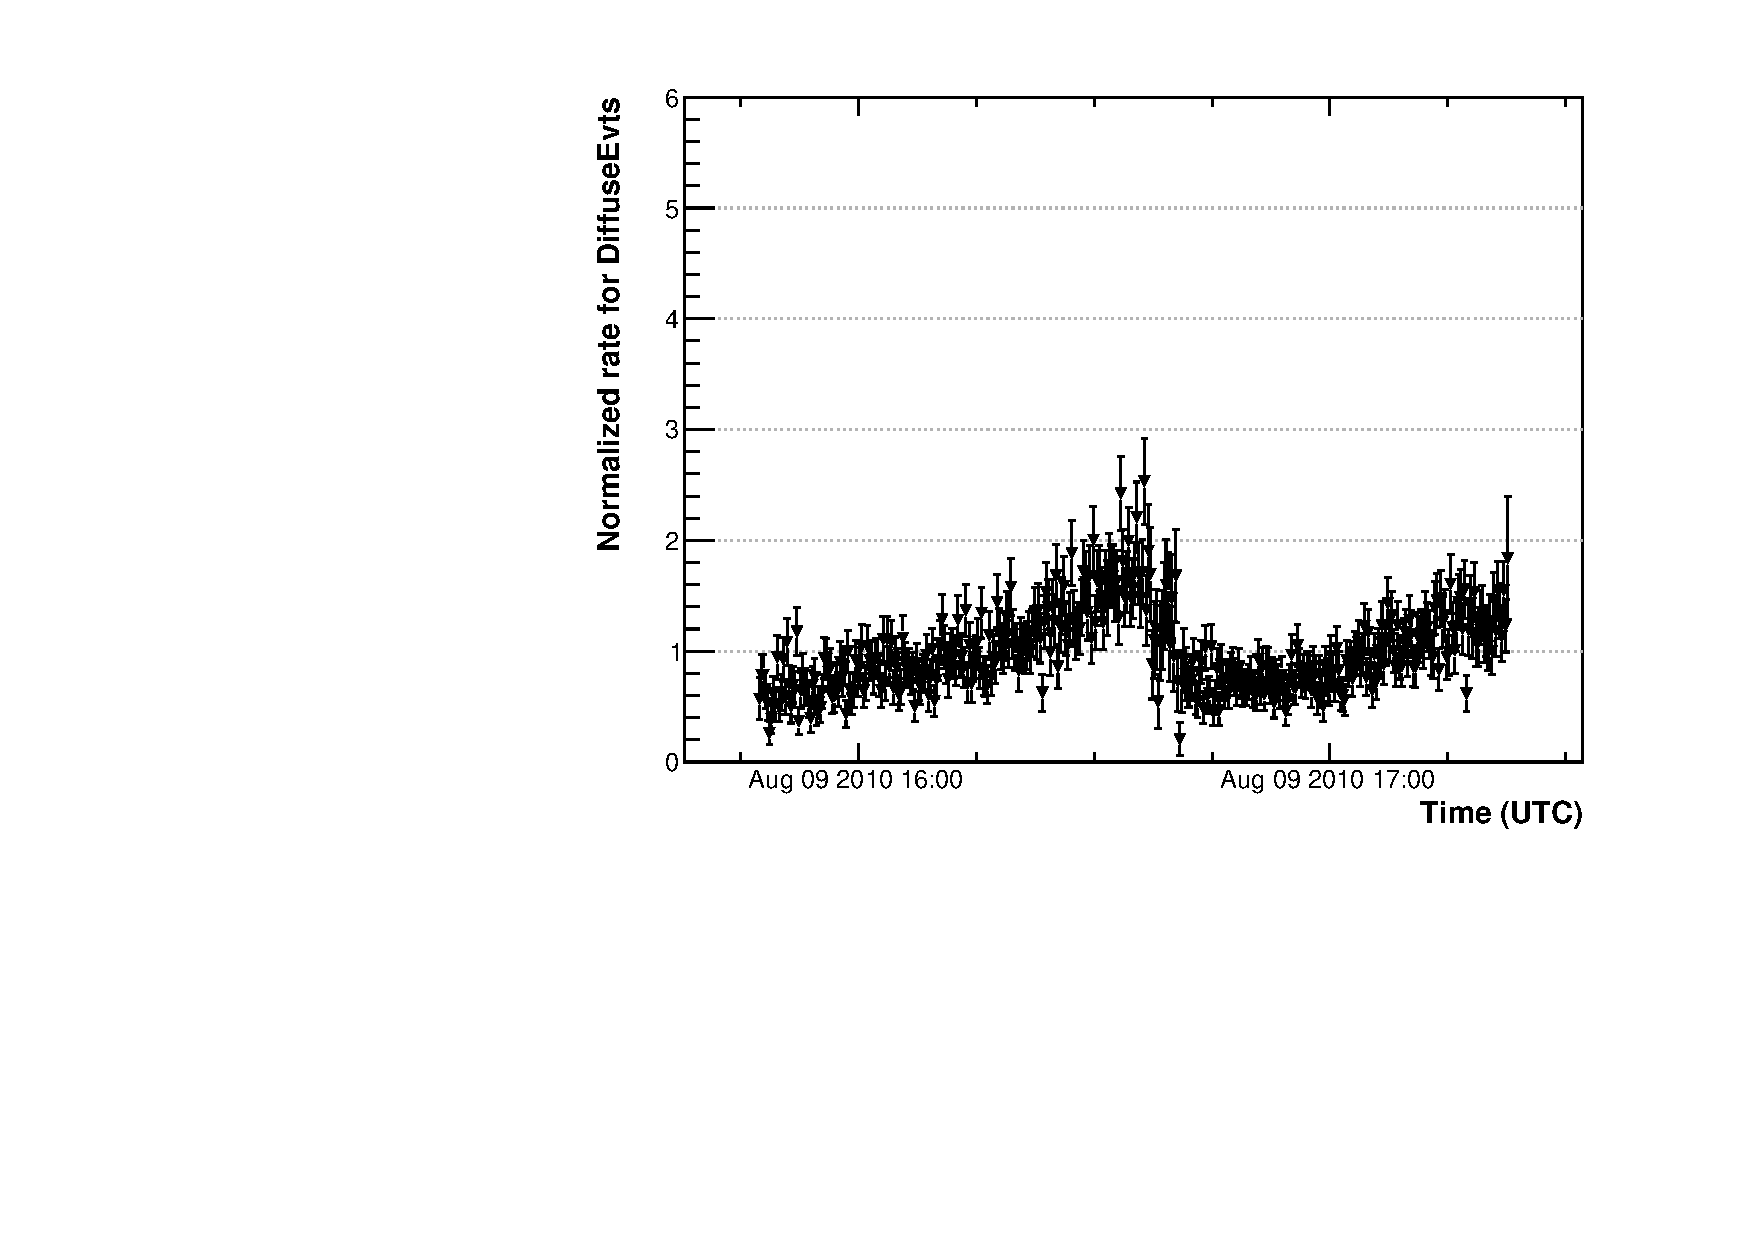
\includegraphics[width=\linewidth]{figures/DiffuseEvts_new}
    \caption{New normalized rate for the diffuse class events for run
      0303054436 (compare with figure \ref{DiffuseEvts_old}).
      The spike in much less prominent with the new algorithm.}
    \label{DiffuseEvts_new}
  \end{center}
\end{figure}


\section{The longitude modulation}

The last issue is the recurrent dip in normalized rate (after the McIwain L and
the Earth limb corrections) in the background-dominated classes.
It appears that, among all the geographic or geomagnetic variables, such dip
feature the highest correlation with the geographic longitude
(cfr. figure \ref{EvtsBeforeCuts_lon}).
\begin{figure}[htb!]
  \begin{center}
    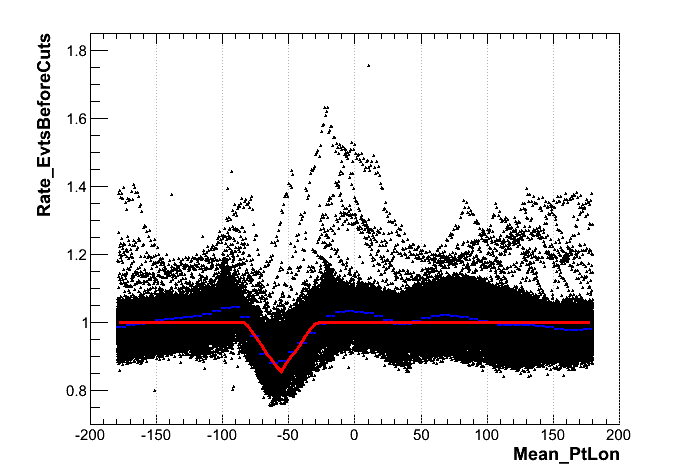
\includegraphics[width=\linewidth]{figures/EvtsBeforeCuts_lon}
    \caption{Dependence of the normalized rate of events before the cuts
      on the geographic longitude.}
    \label{EvtsBeforeCuts_lon}
  \end{center}
\end{figure}

The correlation is fitted with a triangular function:
\begin{equation}
  f(\theta_r) = \min\left(1, 1 - c_0 + c_0 |c_2 (x - c_1)|\right)
\end{equation}
where $c_0$ (the amplitude of the variation) is of the order of 15\% for
event rate before any cut and is much less pronounced for the photon-rich
classes---for which, in fact, it is disengaged.

The effect of such a correction is shown in figure \ref{EvtsBeforeCuts_new},
which can be compared directly with the original implementation (in which
such a correction was not applied) in figure \ref{EvtsBeforeCuts_old}.
\begin{figure}[htb!]
  \begin{center}
    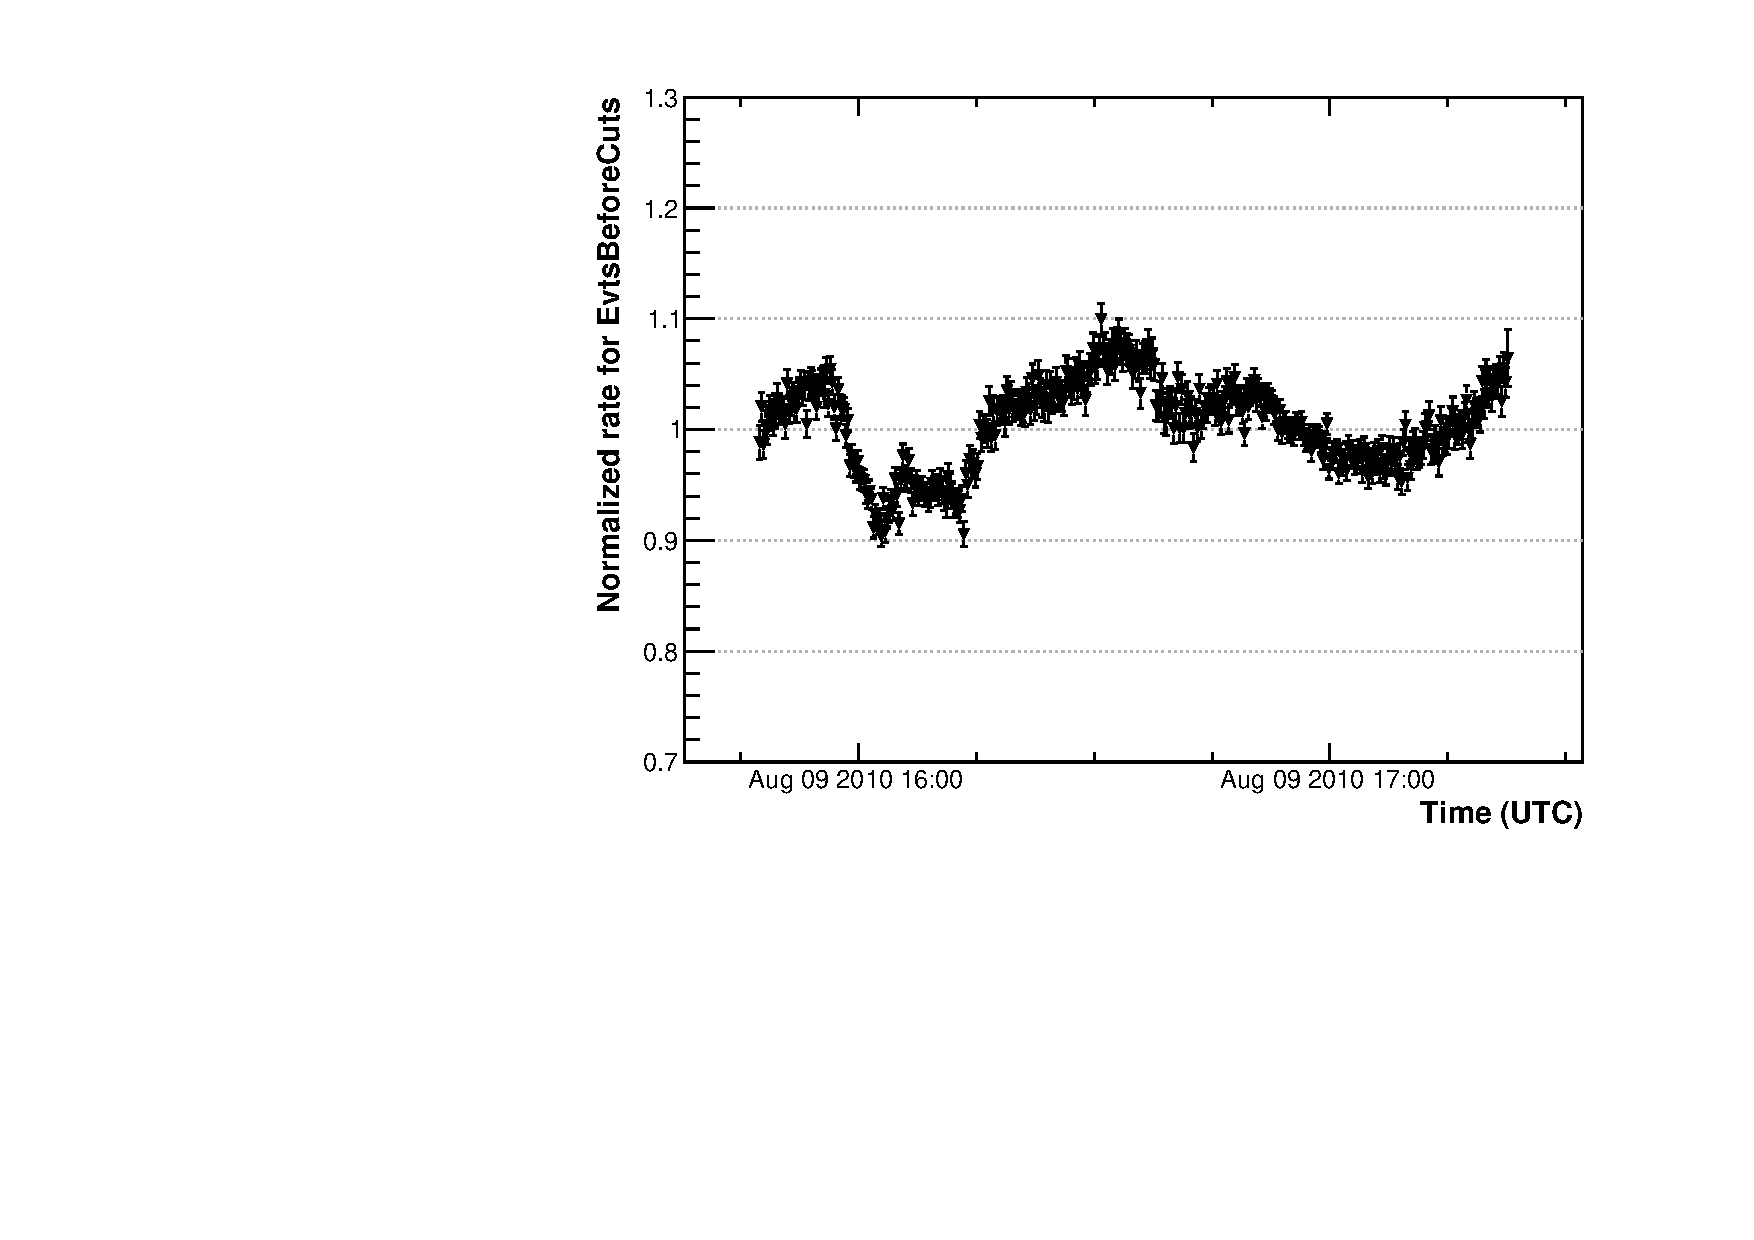
\includegraphics[width=\linewidth]{figures/EvtsBeforeCuts_new}
    \caption{New normalized rate for the events before any cut for run
      0303054436, after the longitude correction has been applied (cfr.
      figure \ref{EvtsBeforeCuts_old}).}
    \label{EvtsBeforeCuts_new}
  \end{center}
\end{figure}

After this new correction the overall normalized rate (at least for this run)
is consistent with unity to 10\% and the dip is much less prominent.


\section{Running the code}

All the code needed in order to generate the configuration files for the
rate normalization lives in the cvs area \texttt{dataMonitoring/Tools/python}.
The structure of the code reflects the process through which it was implemented
and therefore the generation of the files involves several steps.

Setting the environment should be fairly easy, as the code does not
really depend on any other package than \texttt{dataMonitoring/Common}.
Assuming that one has checked out the entire \texttt{dataMonitoring} package,
the only requirement is to make sure that the \texttt{PYTHONPATH} environment
variable includes the folder \texttt{dataMonitoring/Common/python}.

\subsection{Merging the trending files}

The first step is the generation of the root file in which the
\texttt{MERITTREND} datamonitoring products for the desired time span
are merged together. This is accomplished by running the\\
\texttt{\small pMeritTrendMerger.py}\\
script on a SLAC machine (i. e. a machine having access to the Fermi
xrootd area).

Right now the script does not accept command line arguments (it might get
better in the future) so one has to edit by hand the final lines of the
script to change the end of the time span (and, optionally, the length of the
time span itself, which is 56 days by default). The script produce two output
files:
\begin{itemize}
  \item \texttt{merit\_norm\_filelist.txt} containing the list of files used
    for the merging process;
  \item \texttt{merit\_norm.root} containing the actual root tree to be used
    for further processing.
\end{itemize}
If you have already a \texttt{merit\_norm\_filelist.txt} in the working
directory make sure you delete it before you run the script (otherwise it will
be reused). The \texttt{merit\_norm.root} file is the file you have to copy over
locally (if you wish) to produce the text configuration files.

\subsection{Processing the file}

The next step is the processing of the merged root file. As mentioned before,
this does not involve any xrootd access and can be done locally:\\
\texttt{> python pMeritTrendProcessor merit\_norm.root}

\noindent This will create, again, two files:
\begin{itemize}
  \item \texttt{FactorsToNormRates\_noEarthLimb.txt}, a text configuration
    files that can be used in the L1Proc, containing the normalization
    factors for the McIlwain L correction;
  \item \texttt{merit\_norm\_proc.root}, a root file containing all the
    McIlwain L histograms and the full merged tree, processed and normalized
    for the McIlwain L correction.
\end{itemize}

The file \texttt{FactorsToNormRates\_noEarthLimb.txt} should be copied
to\\
\texttt{dataMonitoring/DigiReconCalMeritCfg}\\
and committed in that cvs area.

\subsection{Post-processing the file}

The final step is the correction for the Earth limb and the geographic
longitude:\\
\texttt{> python pMeritTrendPostProcessor merit\_norm\_proc.root}

The two files created are:
\begin{itemize}
  \item \texttt{FactorsToNormRates\_EarthLimb.txt}, the full text configuration
    files---including all the corrections;
  \item \texttt{merit\_norm\_postproc.root}, a root file containing all the
    McIlwain L histograms, all the correction functions and the full merged
    tree, processed and normalized for McIlwain L, Earth limb and longitude.
\end{itemize}

The file \texttt{FactorsToNormRates\_EarthLimb.txt} is ready be copied
to\\
\texttt{dataMonitoring/DigiReconCalMeritCfg}\\
and committed/tagged.


\end{document}
